\documentclass[11pt, reqno]{article} %{amsart} 
\usepackage{geometry}                % See geometry.pdf to learn the layout options. There are lots.
\geometry{letterpaper}                   % ... or a4paper or a5paper or ...
% \geometry{landscape}                % Activate for for rotated page geometry
% \usepackage[parfill]{parskip}    % Activate to begin paragraphs with an empty
% line rather than an indent
\usepackage{graphicx}
\usepackage{amssymb}
\usepackage{amsmath}
\usepackage{epstopdf}
\usepackage{amsmath}
\usepackage{listings}
\usepackage{authblk}
\usepackage[colorlinks=true]{hyperref}
\usepackage{xcolor}

\usepackage{listings}               %Programmcodeumgebung f�r Matlab Code 
\usepackage{microtype}            %Captions im Programmcode 

\hypersetup{bookmarksopen=true}

\definecolor{bgcolor}{rgb}{0,0,0} 
\definecolor{string}{rgb}{1,0,0} 
\definecolor{darkblue}{rgb}{0,0,.75} 
\definecolor{darkred}{rgb}{.75,0,0} 
\definecolor{darkgreen}{rgb}{0,.75,0} 
\definecolor{deepblue}{rgb}{0,0,0.5}
\definecolor{deepred}{rgb}{0.6,0,0}
\definecolor{deepgreen}{rgb}{0,0.5,0}

% Matlab environment
\lstloadlanguages{Matlab} 
\lstnewenvironment{MatlabCode}[1][] 
{\microtypesetup{activate=false}      %Captions im Programmcode 
\lstset{ 
   language=Matlab, 
   basicstyle=\ttm,                     %generell Schreibmaschinenschrift 
%   basicstyle=\scriptsize, 
   keywordstyle=\color{darkblue}, 
   commentstyle=\color{darkgreen}, 
   stringstyle=\color{string}, 
   showstringspaces=false,                  %In Strings keine Backspace zeichen breaklines=true, 
   captionpos=b,                                 %Beschriftungsposition 
   numbers   =   left,                              %links Zeilennummern 
   xleftmargin=.04\textwidth, 
   #1} 
} 
{} 

% Python environment
\DeclareFixedFont{\ttb}{T1}{txtt}{bx}{n}{11} % for bold
\DeclareFixedFont{\ttm}{T1}{txtt}{m}{n}{11}  % for normal

\lstloadlanguages{Python} 
\lstnewenvironment{PythonCode}[1][]
{\microtypesetup{activate=false}      %Captions im Programmcode 
\lstset{
   language=Python, 
   basicstyle=\ttm, 
%  basicstyle=\scriptsize, 
   keywordstyle=\ttb\color{deepblue}, 
%   commentstyle=\color{darkgreen}, 
   emph={MyClass,__init__},          % Custom highlighting
   emphstyle=\ttb\color{deepred},    % Custom highlighting style
   stringstyle=\color{deepgreen}, 
   showstringspaces=false,                  %In Strings keine Backspace zeichen breaklines=true, 
   captionpos=b,                                 %Beschriftungsposition 
   numbers   =   left,                              %links Zeilennummern 
   xleftmargin=.04\textwidth, 
   #1} 
%   language=Python,
%   basicstyle=\ttm,
%   keywordstyle=\ttb\color{deepblue},
%   emph={MyClass,__init__},          % Custom highlighting
%   emphstyle=\ttb\color{deepred},    % Custom highlighting style
%   stringstyle=\color{deepgreen},
%   #1}
}
{}

\usepackage{todonotes}


% Absatz Format: (kein Einruecken)
\parindent 0pt
\parskip 5pt

%\usepackage[sort&compress]{natbib}
%\bibliographystyle{decsci}

\renewcommand{\baselinestretch}{1.1} 

\DeclareGraphicsRule{.tif}{png}{.png}{`convert #1 `dirname #1`/`basename #1 .tif`.png}
\newcommand\numberthis{\addtocounter{equation}{1}\tag{\theequation}}

\newcommand{\etal}{{\textit{et al.}}}
\newcommand{\mle}{\widehat{\theta^i}}
\newcommand{\dbyd}[2]{\frac{\partial #1}{\partial #2}}
\newcommand{\doref}{ {\color{red} refs...}}
\newcommand{\bb}[1]{\mathbb{#1}}
\newcommand{\bs}[1]{\boldsymbol{#1}}
%\newcommand{\bf}[1]{\mathbf{#1}}

\DeclareMathOperator{\cov}{cov}

% Crop figures: for F in `ls S*.pdf`; do pdfcrop $F $F; done

\begin{document}

% \title{LNA++, Feigelman et al.}{Supplementary Materials:  LNA++: a fast C++
% implementation of the Linear Noise Approximation with First and Second Order Sensitivities}
\title{Documentation of LNA++}


\author[1,2,3]{Justin Feigelman}
\author[2]{Daniel Weindl}
\author[1,2]{Fabian J. Theis}
\author[1,2]{Jan Hasenauer}
\author[1]{Carsten Marr}
\affil[1]{Helmholtz Zentrum M\"unchen - German Research Center for Environmental Health, Institute of Computational Biology, Ingolst\"adter Landstra{\ss}e 1, 85764 Neuherberg Germany}
\affil[2]{Technische Universit\"at M\"unchen, Center for Mathematics, Chair of Mathematical Modeling of Biological Systems, Boltzmannstra{\ss}e 3, 85748
Garching, Germany}
\affil[3]{ETH Z\"urich, Institute of Molecular Systems Biology, Auguste-Piccard-Hof 1, 8093 Z\"urich, Switzerland}

% authors and title to pdf meta-data
\makeatletter
\hypersetup{pdftitle={\@title},pdfauthor={\@author}}
\makeatother
 
\date{} % no date
\maketitle
\tableofcontents

%%

\newpage
\section{Toolboxes for Linear Noise Approximation}

LNA++ is a tool designed to efficiently compute the linear noise approximation to a chemical reaction network, along with the first and second order sensitivities of the mean, covariance and temporal cross-covariance matrix. Furthermore, LNA++ facilitates parameter inference on time series data by providing first and second order sensitivities of the log-likelihood with respect to model parameters. To ensure computational efficiency, the numerical simulation is implemented in C/C++.  LNA++ can be either be integrated into a C++ project, or used in conjunction with Matlab or Python for parameter inference in chemical reaction networks.  

This document provides the mathematical background and describes the library requirements, the installation and the usage of LNA++.

\section{Mathematical background}
\subsection{Notation}
Throughout this document we will indicate matrices using double struck notation, and vectors using boldface; time derivatives are indicated using the conventional dot notation, i.e.\ $\dot{x} := \frac{d}{dt}x(t)$. 

\subsection{Chemical reaction networks}
We define a chemical reaction network (CRN) to be a set of chemical reactions defined for a set of chemical species.  Each reaction consumes a set of educts and yields a set of products. Consider a CRN with $R$ reactions, denoted $\mathcal{R}_1, \ldots, \mathcal{R}_R$, between a set of $N$ chemical species. The $j^{th}$ reaction, $\mathcal{R}_j$, can be summarized succinctly as 
\begin{equation}
\mathcal{R}_j: \sum_{i=1}^{N} \bb S_{ij}^{-} X_i \longrightarrow \sum_{i=1}^{N} \bb{S}_{ij}^{+} X_i.
\end{equation}
The matrices $\bb{S}^- = \{\bb{S}_{ij}^-\}$ and $\bb{S}^+=\{\bb{S}_{ij}^+\}$, with $i=1,\ldots,N$ and $j=1,\ldots,R$ denote the stoichiometric matrix of educts and products, i.e.\ the number of molecules of each species consumed or produced in each reaction, respectively. The net stoichiometric matrix is defined as $\bb{S} := \bb{S}^+ - \bb{S}^-$.

\subsection{Linear Noise Approximation}
In the linear noise approximation, the stochastic system dynamics of the CRN are approximated by a set of ordinary differential equations which capture the evolution of the mean and temporal cross-covariance of all species of the CRN.  The molecular copy number $X_i$ of the $i^{th}$ species can be converted to a molecular concentration, denoted $x_i$, by dividing by the size of the reaction volume $\Omega$, such that $x_i=X_i/\Omega, i=1,\ldots,N$. In the following we summarize the LNA for CRNs, for more details see, e.g.\ Van Kampen \cite{VanKampen:2007vu} and Komorowski \etal~\cite{Komorowski:2009hj,Komorowski:2011cn}. 
In the LNA, the molecular concentration vector of the system $\mathbf x(t)=(x_1(t), \ldots, x_N(t))^T$ is approximated by the sum of a deterministic mean term $\bs \phi(t)$ and a stochastic fluctuation term $\bs \eta(t)$:
\begin{equation}
\mathbf x(t) = \bs\phi(t) + \bs\eta(t).
\end{equation}

The deterministic component $\bs\phi(t)$ satisfies the macroscopic rate equations (MRE):
\begin{equation}
\dot{\bs\phi}(t) = \bb{S} \mathbf F(\bs\phi, \bs\Theta, t) \label{eq:MRE}
\end{equation} 
where $\mathbf F =  (F_1,...,F_R)^T$ is the vector of reaction fluxes for each of the R reactions at time $t$ parametrized by model parameters $\bs \Theta = (\theta_1, \ldots, \theta_P)$. The stochastic fluctuation term $\bs \eta(t)$ obeys the stochastic differential equation:
\begin{equation}
d\bs\eta = \bb A(\bs\phi,\bs\Theta,t)\bs\eta\,dt + \bb E(\bs\phi,\bs\Theta,t)d\mathbf{W}
\end{equation}
with
\begin{eqnarray}
\bb A(\bs\phi, \bs\Theta, t) &=& \bb S \dbyd{}{\bs\phi} \mathbf F(\bs\phi,\bs\Theta,t) \label{eq:defA}\\
\bb E(\bs\phi, \bs\Theta, t) &=& \bb S
\sqrt{\text{diag}(\mathbf F(\bs\phi,\bs\Theta,t))}
\end{eqnarray}
where $\mathbf{W}$ is a $N$-dimensional Wiener process. The covariance of the system at time $t$, $\bb V(t) = \text{cov}(\mathbf x(t) )$, i.e.\ $\bb V$ is the matrix with entries $\bb{V}_{ij}(t) = \cov(\mathbf{x}_i(t), \mathbf{x}_j(t))$, is given by the solution of
\begin{equation}
\dot{\bb V}(t)= \bb A \bb V+ \bb V \bb A^T + \bb E \bb E^T.\label{eq:variance}
\end{equation}
Temporal cross-covariances $\text{cov}(\mathbf x(s),\mathbf x(t))$ between
the system at times $s$ and $t, t \geq s$, are derived by applying the fundamental
solution matrix $ \bb{G}(s,t)$, defined by \eqref{eq:fund_RE}, to the system
variance at time s:
\begin{eqnarray}
\text{cov}\left(\mathbf x(s), \mathbf x(t)\right) &=& \bb V(s)
 \bb{G}(s,t)^T \label{eq:cov_LNA} \label{eq:CovarianceODE}\\
\dot{\bb{G}}(s,t) &=& \bb A \bb{G}(s,t)
\label{eq:fund_RE}
\\
\bb{G}(s,s) &=& \bb I_N.\label{eq:fund_RE_identity}
\end{eqnarray}

The variance $\mathbb{V}$ and the temporal cross-covariance $\cov(\mathbf x(s),\mathbf x(t))$ can be employed to evaluate the correlation of the system across multiple time points. We denote the vector of stacked states at different time points $t_1,\ldots,t_M$ by
\begin{equation}
\tilde{\mathbf{x}} =
(x_1(t_1),...,x_N(t_1),x_1(t_2),...,x_N(t_2),...,x_1(t_M),...,x_N(t_M))^T. \label{eq:stackedX}
\end{equation}
The covariance of $\tilde{\mathbf{x}}$ is given by the temporal cross-covariance block matrix $\Sigma = \{\Sigma^{kl}\}_{k,l=1}^M$. In matrix notation we obtain
$$
\Sigma = \cov(\tilde{\mathbf x}) = \left(
\begin{array}{cccc}
\bb{V}(t_1) & \cov(\mathbf{x}(t_1),\mathbf{x}(t_2)) & ... & \cov(\mathbf{x}(t_1),\mathbf{x}(t_M)) \\
\cov(\mathbf{x}(t_2),\mathbf{x}(t_1)) & \bb{V}(t_2) & ... & \cov(\mathbf{x}(t_2),\mathbf{x}(t_M)) \\
\vdots & \vdots & \ddots & \vdots \\
\cov(\mathbf{x}(t_M),\mathbf{x}(t_1)) & \cov(\mathbf{x}(t_N),\mathbf{x}(t_2)) &
... & \bb{V}(t_M) \\
\end{array}
\right) .$$

The temporal cross-covariance block matrix is constructed by setting $\Sigma^{kk}=\bb{V}(t_k), k=1,\ldots,M$, along the diagonal, and
\begin{equation}
\begin{aligned}
\label{eq:BlockCovariance}
\Sigma^{kl} & = \cov(\mathbf x(t_k), \mathbf x(t_l)) \\
	& = \bb{V}(t_k)\bb{G}(t_k,t_l)^T,k<l\leq M
\end{aligned}
\end{equation}
for the off-diagonal elements.

\subsection{Computing the likelihood of a trajectory}
The likelihood of a trajectory $\tilde{\mathbf{x}}$ as defined in \eqref{eq:stackedX} consisting of observations at $M$ discrete time points, conditional on the model parameters $\bs \Theta$, is given by a multivariate normal distribution with stacked mean $\tilde{\bs{\phi}}=(\bs \phi_1(t_1),\ldots,\bs \phi_N(t_1),\ldots, \bs \phi_1(t_M),\ldots,\bs \phi_N(t_M))^T$ obtained by solving \eqref{eq:MRE}, and cross-covariance matrix $\Sigma$ computed via
\eqref{eq:variance}, and \eqref{eq:CovarianceODE}. The likelihood of $\bs \Theta$ is given by:
\begin{equation} 
\label{eq:LNAlikelihood}
L(\bs{\Theta}) = P(\tilde{\mathbf x} | \bs{\Theta}) = \left(2\pi\right)^{-M/2} |\Sigma|^{-1/2} \exp\left\{ -\frac{1}{2} (\tilde{\mathbf x} - \tilde{\bs \phi})^T \Sigma^{-1} (\tilde{\mathbf x} - \tilde{\bs \phi}) \right\}
\end{equation}
where $\vert \Sigma \vert$ denotes the determinant of $\Sigma$, and $\phi$, $\Sigma$ are functions of $\bs \Theta$.
Similarly, the log-likelihood of $\bs \Theta$,
$\ell(\bs \Theta) := \log L(\bs \Theta)$, is given by:
\begin{equation}
\ell (\bs \Theta) = -\frac{N}{2} \log(2\pi) -\frac{1}{2} \log |\Sigma| -\frac{1}{2} (\tilde{\mathbf x} - \tilde{\bs \phi})^T\Sigma^{-1}(\tilde{\mathbf x} - \tilde{\bs\phi})
\end{equation}

\subsection{First order sensitivities}
\subsubsection{Analytical}
The sensitivity of the log-likelihood with respect to the $k^{th}$ model parameter, $\theta_k$, is given by $\frac{d \ell}{d \theta_k}$. For the following we introduce the shorthand notation $\phi'_i := \frac{d}{d \theta_i} \phi$, $\phi''_{ij} := \frac{d^2}{d\theta_i d\theta_j} \phi$, and similarly for all components of the LNA.

The first order sensitivity of the log-likelihood with respect to $\theta_i$ is
computed as:
\begin{equation}
\begin{aligned}
\frac{d \ell}{d \theta_i}  
	&=-\frac{1}{2}\frac{d \log|\Sigma|}{d \theta_i}  
	-\frac{1}{2} \left(
		( - \tilde{\bs\phi}'_i )^T \Sigma^{-1}(\tilde{\mathbf x} - \tilde{\bs\phi}) + 
		(\tilde{\mathbf x} - \tilde{\bs \phi})^T \frac{d \Sigma^{-1}}{d
		\theta_i}(\tilde{\mathbf x} - \tilde{\bs \phi}) + (\tilde{\mathbf x} -
		\tilde{\bs \phi})^T\Sigma^{-1}(-\tilde{\bs\phi}'_i)  \right) \\
		& = -\frac{1}{2}\text{Tr}\left(\Sigma^{-1}\Sigma'_i\right)
		  + (\tilde{\bs\phi}'_i)^T\Sigma^{-1}(\tilde{\mathbf x} - \tilde{\bs\phi}) 
		  + \frac{1}{2} (\tilde{\mathbf x} -\tilde{\bs\phi})^T\left(\Sigma^{-1}
		  \Sigma'_i\Sigma^{-1}\right)(\tilde{\mathbf x}-\tilde{\bs\phi}) 
\end{aligned}
\end{equation}
where $\Sigma'_k$ and $\bs\phi'_k$ are computed using the forward sensitivity equations below in conjunction with \eqref{eq:MRE} and
\eqref{eq:cov_LNA}:
\begin{eqnarray}
\dot{\bs\phi'_k}(t) &=& \frac{d}{d \theta_k} \dot{\bs\phi}(t)
 =  \bb{S} \frac{d}{d \theta_k} \mathbf F(\bs \phi,\bs{\Theta},t)
 \\
 &=& \bb{S} \left(\frac{\partial \mathbf F}{\partial \bs \phi}
 \bs \phi'_k + \frac{\partial \mathbf F}{\partial \theta_k}\right) \label{eq:MRE_sensitivity} \\ 
 &=& \bb{A} \phi'_k + \bb{S} \dbyd{\mathbf F}{\theta_k }\\
\frac{d}{d \theta_k} \cov \left(\mathbf x(s), \mathbf x(t)\right) &=& \bb{V}'_k  \bb{G}(s,t)^T + \bb V(s) \bb{G}'_k(s,t)^T \label{eq:Var_sensitivity} \\
\dot{\bb{V}}'_k &=& \frac{d}{d\theta_k} \dot{\bb V}(t) = \bb{A}'_k \bb V + \bb A \bb{V}'_k +
	\bb{V}'_k \bb A^T + \bb V {\bb{A}'_k}^T +
	\bb{E}'_k \bb E^T + \bb E {\bb{E}'_k}^T \label{eq:Variance_sensitivity}
\end{eqnarray}

The partial derivatives $\frac{\partial V(s)}{\partial \theta_k}$ and $\frac{\partial \bb{G}(s,t)}{\partial \theta_k}$ are computed by differentiating Equations \ref{eq:variance} and \ref{eq:fund_RE}, respectively, with respect to $\theta_k$, and numerically integrating the ODE system for $\frac{d}{dt} \frac{\partial V}{\partial \theta_k}$, $\frac{d}{dt} \frac{\partial \bb{G}}{\partial \theta_k}. $ 

\subsubsection{Finite difference approximation}
\label{sec:FirstOrderFD}
The forward finite difference approximation of a function $f(\theta)$ is obtained by Taylor expanding the function about the point $\theta$:
\begin{equation}
\label{eq:FirstOrderFD}
f(\theta+\Delta \theta) = f(\theta) + f'(\theta) \Delta \theta  +
\mathcal{O}(\Delta \theta ^2).
\end{equation}
Ignoring terms with power of $\Delta \theta$ greater than one, $f'(\theta) \approx \frac{f(\theta+\Delta \theta) - f(\theta)}{\Delta \theta}.$ Thus the computation of the finite difference approximation requires one additional evaluation of $f$ at $\theta + \Delta \theta$. Likewise, for a function $f(\bs\Theta), \bs \Theta \in \bb R^d$, the finite difference approximation to the gradient $\nabla_{\bs \Theta} f$ requires an additional $d$ evaluations of $f$.

\subsection{Second order sensitivities}
\subsubsection{Analytical}
The matrix of second order sensitivities, i.e.\ the Hessian, of the log-likelihood is computed as $\frac{\partial^2 \ell}{\partial \bs \Theta^2} = \{\frac{\partial^2 \ell}{\partial \theta_i \partial \theta_j}\}_{i,j=1}^d$, where the $(i,j)^{\text{th}}$ term is given by
\begin{equation}
\begin{aligned}
\frac{d^2 \ell}{d \theta_i d \theta_j}  & = -\frac{1}{2} \text{Tr} \left(
-\Sigma^{-1} \Sigma'_j \Sigma^{-1} \Sigma'_i + \Sigma^{-1} \Sigma''_{ij} \right)
+  (\tilde{\bs\phi}''_{ij})^T \Sigma^{-1} \left(\tilde{\mathbf x}-\tilde{\bs\phi}
\right)
\\
	& - (\tilde{\bs\phi}'_i)^T \left( \Sigma^{-1} \Sigma'_j
	\Sigma^{-1} \right) (\tilde{\mathbf x}-\tilde{\bs\phi}) - \tilde{\bs\phi'_i}^T
	\Sigma^{-1}\tilde{\bs\phi}'_j - ({\tilde{\bs\phi}'_j})^T(\Sigma^{-1} \Sigma'_i
	\Sigma^{-1})(\tilde{\mathbf x} - \tilde{\bs\phi}) \\
	& + \frac{1}{2}(\tilde{\mathbf x}-\tilde{\bs\phi})^T  \Sigma^{-1} ( - 2
	\Sigma'_j \Sigma^{-1} \Sigma'_i  + \Sigma''_{ij} ) \Sigma^{-1} (\tilde{\bf x} -
	\tilde{\bs \phi}) \label{eq:Hessian} .
\end{aligned}
\end{equation}
It depends on the higher order sensitivities of the macroscopic rate equation ($\bs \phi''_{ij}$) and of the temporal cross-covariance matrix ($\Sigma''_{ij}$). Recalling the equations for the first order sensitivities \eqref{eq:MRE_sensitivity}, \eqref{eq:Var_sensitivity} and \eqref{eq:defA}, we find that the second order sensitivity of the MRE ($\bs\phi''_{ij}$) is given by:
\begin{eqnarray}
\dot{\bs \phi}''_{ij} &=& \frac{d}{d \theta_j}\dot
{\bs\phi}'_i(t) \nonumber \\
	&=& \bb{A}'_j \bs\phi'_i + \bb A \bs\phi''_{ij} + \bb
	S  \frac{d}{d \theta_j} \frac{\partial \mathbf F}{\partial \theta_i} \nonumber \\
	&=& \left( \dbyd{\bb A}{\bs\phi} \bs \phi'_j + \frac{\partial \bb A}{\partial \theta_j} \right) \bs\phi'_i + \bb A \bs\phi''_{ij} + 
		\bb{S} \left( \dbyd{}{\bs \phi}\frac{\partial \mathbf F}{\partial \theta_i} \dbyd{\bs \phi}{\theta_j}+ 
		\frac{\partial}{\partial \theta_j}\frac{\partial \mathbf F}{\partial
		\theta_i} \right) \nonumber \\
	&=& \left( \dbyd{\bb A}{\bs\phi} \bs\phi'_j + \frac{\partial \bb A}{\partial \theta_j} \right) \bs\phi'_i + \bb A \bs\phi''_{ij} + 
		 \frac{\partial \bb A}{\partial \theta_i} \bs\phi'_j + \bb{S} \frac{\partial^2
		 \mathbf F}{\partial \theta_j \partial \theta_i} .
\end{eqnarray}		
The computation of the second order sensitivities of the temporal cross-covariance matrix is slightly more involved, and requires also the higher order sensitivities of the fundamental matrix ($\bb{G}''_{ij}$). From \eqref{eq:cov_LNA}-\eqref{eq:fund_RE_identity} we find
\begin{equation}		
\frac{d}{d \theta_i}\text{cov}(\mathbf x(s), \mathbf x(t)) = \bb{V}'_i(s) \bb{G}^T(s,t) + \bb V(s) {\bb{G}'_i}^T(s,t)
\end{equation} 
and
\begin{equation}
\frac{d ^2}{d \theta_i d \theta_j} \cov(\mathbf x(s), \mathbf x(t)) = \bb{V}''_{ij}(s) \bb{G}^T(s,t) +
	\bb{V}'_i(s) {\bb{G}'_j}^T(s,t) + \bb{V}'_j(s) {\bb{G}'_i}^T(s,t) + \bb V(s) {\bb{G}''_{ij}}^T(s,t) .
\end{equation}
From \eqref{eq:Variance_sensitivity} we find
\begin{eqnarray}
\dot{\bb{V}''}_{ij}(t) &= & \frac{d}{d \theta_j}\dot{\bb{V}'}_i \nonumber \\
	&=& 
	\begin{aligned} 
		& \bb{A}''_{ij} \bb V + \bb{A}'_i \bb{V}'_j + \bb{A}'_j \bb{V}'_i + \bb A \bb{V}''_{ij}   
		+ \bb{V}''_{ij} \bb A^T + \bb{V}'_i \bb{A}'_j  \\
		& + \bb{V}'_j {\bb{A}'_i}^T + \bb V
		 (\bb{A}''_{ij})^T +  \bb{E}''_{ij} \bb E^T
		 + \bb{E}'_i + {\bb{E}'_j}^T + \bb{E}'_j
		 (\bb{E}'_i)^T + \bb E (\bb{E}''_{ij})^T 
	\end{aligned} \\
\bb{A}''_{ij} &=& \frac{d}{d\theta_j} \left( \frac{\partial\bb{A}}{\partial \bs \phi} \bs\phi'_i + \frac{\partial \bb{A}}{\partial \theta_i} \right) \nonumber \\
	&=& \left( \frac{\partial^2 \bb{A}}{\partial \bs{\phi}^2} \bs{\phi}'_j + \frac{\partial^2 \bb{A}}{\partial \theta_j \partial \bs{\phi}} \right) \bs{\phi}'_i
	+ \frac{\partial \bb{A}}{\partial \bs{\phi}} \phi''_{ij} 
	+ \frac{\partial}{\partial \bs{\phi}} \frac{\partial \bb{A}}{\partial \theta_i} \frac{\partial \bs{\phi}}{\partial \theta_j}
	+ \frac{\partial^2 \bb{A}}{\partial \theta_j \partial \theta_i}.
\end{eqnarray}
The sensitivities of the fundamental matrix $\bb{G}$ are computed using \eqref{eq:CovarianceODE}:
\begin{eqnarray}
\dot {\bb{G}}'_i(s,t)  &=& \bb{A}'_i(t) \bb{G}(s, t) + \bb A(t) \bb{G}'_i(s,t) \\
\dot{\bb{G}}''_{ij}(s,t)  &=&\bb{A}''_{ij}(t) 
\bb{G}(s,t) + \bb{A}'_i(t)   \bb{G}'_j(s,t) + \bb{A}'_j(t)  \bb{G}'_i(s,t) + \bb A \bb{G}''_{ij}(s,t).
\end{eqnarray}

\subsubsection{Finite difference approximation}
\label{sec:SecondOrderFD}
Consider a function $f(\bs \Theta)$, where $\bs \Theta = (\theta_1,\ldots,\theta_d)^T$.
The finite difference approximation of the second order sensitivity of $f(\bs\Theta)$ with respect to the $(i,j)^{\text{th}}$ model parameters, $\frac{\partial^2 f}{\partial \theta_i \partial \theta_j}$, can be numerically computed using the following Taylor expansion about $\bs \Theta$ with small perturbations $\Delta \theta_i$ and $\Delta \theta_j$:

\begin{equation}
\label{eq:SecondOrderFD}
\begin{split}
\frac{\partial^2 f(\boldsymbol{\Theta})}{\partial \theta_i \partial \theta_j} \approx 
\frac{1}{2\Delta \theta_i \Delta \theta_j} 
 \bigg[
	f(\boldsymbol{\Theta} + \mathbf{e_i} \Delta \theta_i + \mathbf{e_j} \Delta \theta_j)
	- f(\boldsymbol{\Theta} + \mathbf{e_i} \Delta \theta_i) 
	- f(\boldsymbol{\Theta} + \mathbf{e_j} \Delta \theta_j) \\
	+ 2f(\boldsymbol{\Theta}) 
	- f(\boldsymbol{\Theta} - \mathbf{e_i} \Delta \theta_i)
	- f(\boldsymbol{\Theta} - \mathbf{e_j} \Delta \theta_j)
	+ f(\boldsymbol{\Theta} - \mathbf{e_i} \Delta \theta_i - \mathbf{e_j} \Delta \theta_j) \bigg] 
\end{split}
\end{equation}
where $\mathbf{e_i}$ indicates the vector of zeros with a one in the $i^{th}$ position.
Thus the computation of the finite difference approximation \eqref{eq:SecondOrderFD} requires an additional 6 evaluations of the 
function $f(\bs \Theta)$ (two of which are shared with the first order finite difference approximation).


\subsubsection{Confidence intervals of parameter estimates}
Confidence intervals can be computed using the maximum likelihood estimator (MLE) and the Hessian of the log-likelihood computed in \eqref{eq:Hessian}. In particular, using the Hessian, it is possible to make the Laplace approximation to the probability density function (pdf) of the model parameters, i.e.\ approximating the pdf as a multivariate Gaussian locally around the MLE. The mean is given by the MLE $\hat{\bs \Theta}$, and the covariance matrix by the negative inverse Hessian, evaluated at $\hat{\bs \Theta}$:
\begin{equation}
\bs \Theta \sim \mathcal{N}\left(\hat{\bs \Theta},
-\left. \left(\dbyd{^2 \ell(\bs{\Theta})}{\bs \Theta^2}  \right)^{-1} \right \rvert_{\bs{\Theta}=\bs{\hat \Theta}}\right)
\label{eq:ConfidenceInterval}
\end{equation}

%
%
%
\section{LNA++ installation and requirements}
\subsection{Installation}
Unpack the LNA++ archive or clone the LNA++ repository which contains all the necessary scripts and source code for building LNA++ Python modules or Matlab executable files. No further building or installation of LNA++ itself is necessary until the creation of the model executables, as described below.

\subsection{Requirements}
LNA++ uses the standard C(++) libraries, the CVODES Sundials library for numerical integration of ODEs and forward sensitivities, and the Blitz++ library for fast, templatized tensor operations. 

\subsubsection*{Compiler}
Compilation of C/C++ source code for use as a standalone executable, or with Matlab or Python requires the use of a suitable compiler such as \texttt{gcc/g++} or \texttt{clang}.

\subsubsection*{Blitz++}
Blitz++ version 1.0.1 is required. This version is included in the \texttt{./libraries} folder. Alternatively, Blitz++ can be downloaded from \href{https://github.com/blitzpp/blitz}{https://github.com/blitzpp/blitz}. It is also available via macports on mac OS. 

When using the provided source archive, extract it to \texttt{../libraries/blitz-1.0.1}, change to this folder and run:\\
\texttt{./configure --with-pic --prefix=`pwd`/../install/blitz-1.0.1 \&\& make install}

For other versions of Blitz++ in non-default locations you need to adapt \texttt{include\_dirs} and \texttt{library\_dirs} in
\texttt{python/setupTemplate.py} or the respective lines in \texttt{matlab/compileLNA.m}.

\subsubsection*{CVODES}
Numerical integration is computed using the CVODES Sundials package.  Source code is included in \texttt{./libraries}, and is also available from \href{http://computation.llnl.gov/casc/sundials}{http://computation.llnl.gov/casc/sundials}.
To setup CVODES, unzip the source archive, change to the source directory and run:

\begin{verbatim}
./configure --with-pic --prefix=`pwd`/../install/cvodes-2.7.0
make && make install
\end{verbatim}

\textit{Note:} CVODES should be compiled using the \texttt{-fPIC} flag to ensure cross-platform compatibility. This can be enabled by specifying \texttt{--with-pic} to the configure script.

\subsubsection*{Python}

In order to use LNA++ with Python, ensure you have installed the necessary scientific computing modules as listed below. Python libraries can be installed using package managers such as apt on Ubuntu, or macports/homebrew on Mac OS, or using the \texttt{pip3} Python package manager.

LNA++ is compatible with Python 3.0 or later.  All libraries must thus be the Python3-compatible version.

\textit{Note for Ubuntu Users:} The necessary Python packages can be installed using the command\\
\texttt{sudo apt install python3-numpy python3-sympy libsbml5-python python3-ipdb}

\begin{description}
 \item[numpy] 
  Numpy is a widely used mathematics and numerical library.
 \item[sympy]
  Sympy provides a framework for symbolic/algebraic computations, and is necessary for computing the linear noise approximation for arbitrary models.
 \item[libsbml]
  Libsbml is required for translating SBML models for use with LNA++.
 \item[ipdb]
  IPython debugger.
 \item[(optional) pylab]
  Pylab provides functions for plotting vectors and matrices, and might thus be useful.
\end{description}


\subsubsection*{Matlab}
In order to use LNA++ with Matlab, the Matlab \textit{Symbolic Math Toolbox} is required for the analytic derivation of the LNA and its sensitivity equations. Matlab is not required when using only the Python version LNA++.

% {DW: I would consider this rather experimental until more testing has been done.}
%\paragraph{If you do not have the \textit{Symbolic Math Toolbox} available:}
%Both the Python and Matlab implementations of LNA++ generate the same C code for the analytical components of the LNA and its sensitivities. It is therefore possible to generate the C code using the Python scripts, through the \texttt{generateLNAComponents} step, as described below. The Matlab executable is then generated in the normal way, resuming with the \texttt{compileLNA} step.

%
%
%
\section{Usage}

In this section we describe how to use LNA++ to create Matlab executable models and Python modules. More application examples are available in the \texttt{examples/} directory.

\subsection{Overview}
LNA++ converts a user-specified model, provided as an SBML model configuration file, into a set of symbolic functions for the time derivatives of means, temporal cross-covariances, and their sensitivities. These functions are converted to C code which is then compiled together with the core computation engine to generate either Matlab or Python executable files/modules. The system can then be simulated using these executables and user-specified initial conditions and model parameters. 

The stoichiometric matrix and reaction propensity functions are extracted from a user-supplied SBML model file (see \href{http://sbml.org/SBML_Software_Guide/SBML_Software_Summary}{http://sbml.org/}) or can be provided directly.

\subsection{Matlab}
To generate the Matlab executable simply call the function \texttt{generateLNA} specifying the path to the SBML input file, the model name and an optional argument indicating whether to attempt to compute the steady state of the system as described below. See also \texttt{examples/runBirthDeath.m} for a detailed example of how this is done.

\subsubsection*{Building the model}
To build the model call \texttt{generateLNA(sbmlFileName, modelName, computeSS)}
\begin{enumerate}
\item \texttt{sbmlFileName}: the path of the SBML model specification file
\item \texttt{modelName}: the desired name of the model 
\item \texttt{computeSS}:  this argument is optional and can have only one of the values \texttt{`Y0'}, \texttt{`V0'}, \texttt{`BOTH'}, or \texttt{`NONE'}.
	\begin{enumerate}
	\item \texttt{`Y0'}:  LNA++ will attempt to calculate the steady state value of the MRE of the stochastic system specified. If \texttt{Y0} is not explicitly provided when invoking the model, the computed value will be automatically substituted. 
	\item \texttt{`V0'}: LNA++ will attempt to calculate the steady state value of the variance of the stochastic system specified. If \texttt{V0} is not explicitly provided when invoking the model, the computed value will be automatically substituted.
	\item \texttt{`BOTH'}: LNA++ will compute both \texttt{V0} and \texttt{Y0} if possible. If \texttt{Y0} or \texttt{V0} is not explicitly provided when invoking the model, the computed values will be automatically substituted.
	\item \texttt{`NONE'}: LNA++ will not compute any steady state values.  Invocation of the model without explicitly specifying the initial conditions for \texttt{Y0} and \texttt{V0} will result in an error message being generated.
	\end{enumerate}
\end{enumerate}

\textit{Note for custom library paths and custom linker or compiler flags:}
It is also possible to specify custom flags to the linker or compiler, for example if CVODES or Blitz are not installed in a standard location.  Linker and compiler flags can be specified using Name, Value argument pairs where Name is either \texttt{Linker\_Flags}, or \texttt{Cpp\_Flags}, e.g.,
\begin{itemize}
\item \texttt{generateLNA(sbmlFileName, modelName, computeSS, `Linker\_Flags', FLAGS)} or
\item \texttt{generateLNA(sbmlFileName, modelName, computeSS, `Cpp\_flags', FLAGS)}.
\end{itemize}
Linker flags and compiler flags can both be specified, by providing both pairs of arguments.


\subsubsection*{Matlab executable}
\texttt{generateLNA} generates a mex file and a Matlab wrapper, which provides help messages and removes singleton dimensions for more convenient output. These are placed in the \texttt{models/} subdirectory with the name of the model as specified in the \texttt{generateLNA} call. To execute them, copy them to the desired final folder, or add them to the Matlab path using \texttt{addpath}. Usage of the generated function is specified in the help for that function.

See \texttt{examples/runBirthDeath.m}, and the generated \texttt{models/BirthDeath/BirthDeath\_LNA.m} for an example of the generated wrapper function and its invocation.

\subsubsection*{Using the generated mex wrapper}
The mex wrapper corresponding to a particular model can be invoked with between 2 and 6 arguments, which must occur in the correct order:

\paragraph{Inputs:}
\begin{enumerate}
\item \texttt{Theta}: the vector of model parameters, with the same dimension as specified during the model construction
\item \texttt{Timepoints}: a vector of times at which the result of the model simulation is to be outputted. The first time is always zero.
\item \texttt{Y0} (optional): a vector of initial conditions for each of the species.  The length must be the same as the number of species.  If omitted, the steady-state initial conditions are assumed, if they were computed when the model was created; otherwise an error is generated requesting the initial conditions to be specified.
\item \texttt{V0} (optional): a vector of initial conditions for the (co-)variances between all species. They are specified in column-major order, i.e. for a 3x3 matrix
\item \texttt{Merr} (optional): a vector of numbers (possibly of length 1) corresponding to estimated measurement error of each species, specified as a variance.  The measurement error is added to diagonal of the temporal cross-covariance matrix.  If only one number is specified, this number is used for all species.  If multiple numbers are specified, the number specified must equal the number of observed variables.  If omitted, measurement error is assumed to be zero for all species.
\item \texttt{obsVar} (optional): a vector of indices corresponding to the species which should be outputted.  The numbering of species matches the numbering of species in the stoichiometric matrix.  If omitted, all species are outputted.
\begin{equation*}
\begin{bmatrix}
\texttt{V\_11},\texttt{V\_12},\texttt{V\_13} \\
\texttt{V\_21},\texttt{V\_22},\texttt{V\_23} \\
\texttt{V\_31},\texttt{V\_32},\texttt{V\_33}
\end{bmatrix}
\end{equation*}
with \texttt{V\_12 = V\_21}, \texttt{V\_13 = V\_31}, and \texttt{V\_23 = V\_32} the initial conditions \texttt{V0} would be specified in the order \texttt{[V\_11,V\_12,V\_22,V\_13,V\_23,V\_33]}. Only the upper triangular portion of the initial covariance matrix is specified due to symmetry.  If omitted, the steady-state values are substituted, if they were computed when the model was created; otherwise an error is generated.

For convenience, the function \texttt{toLinear} is provided as a Matlab script, which converts a symmetric covariance matrix into a column-major-ordered vector.
\end{enumerate}

\paragraph{Outputs:}
If only 2 output arguments are specified, the computation engine does not compute sensitivities, which can be substantially faster.  If 3 or 4 outputs are specified, first order sensitivities are computed.  If 5 or 6 outputs are specified, first and second order sensitivities are computed which can take longer. In the following $N$ is the number of observed variables (\texttt{obsVar}), $T$ is the number of time points specified by \texttt{Time}, and $d$ is the number of model parameters + the number of species \todo{check meaning of $d$}. Note that LNA++ computes sensitivities with respect to model parameters and the initial conditions of the \texttt{MRE}, but not currently with respect to the initial variances.
\begin{enumerate}
\item \texttt{MRE}: a $N \times T$ matrix corresponding to the solution of the macroscopic rate equation for all observed variables.  
\item \texttt{Sigma}: a $N \times N \times T$ array corresponding to the temporal cross-covariance of all observed species at all time points. 
\item \texttt{dMRE} (optional): a $N \times T \times d$ array corresponding to the first order sensitivities of the \texttt{MRE} to each of the model parameters over all time points. The sensitivities are ordered such that the first sensitivities are of the \texttt{MRE} with respect to the model parameters, followed by sensitivities with respect to the initial conditions of each species.
\item \texttt{dSigma} (optional): a $N \times N \times T \times d$ array corresponding to the first order sensitivities of the temporal cross-covariance matrix at all timepoints for the observed species. The sensitivities are ordered such that the first sensitivities are of the \texttt{MRE} with respect to the model parameters, followed by sensitivities with respect to the initial conditions of each species.
\item \texttt{d2MRE} (optional): a $N \times T \times d \times d$ array corresponding to the second order sensitivities of the \texttt{MRE} at all timepoints for the observed species. The sensitivities are ordered such that the first sensitivities are of the \texttt{MRE} with respect to the model parameters, followed by sensitivities with respect to the initial conditions of each species.
\item \texttt{d2Sigma} (optional): a $N \times N \times T \times d \times d$ array corresponding to the second order sensitivities of the temporal cross-covariance matrix at all timepoints for the observed species. The sensitivities are ordered such that the first sensitivities are of the \texttt{MRE} with respect to the model parameters, followed by sensitivities with respect to the initial conditions of each species.
\end{enumerate}

%
\subsection{Python}
To use LNA++ with Python, call the function \texttt{generateLNA} of the LNA module, with the following arguments:
\begin{enumerate}
\item \texttt{sbmlFileName}: the path to the SBML model specification file
\item \texttt{modelName}: the desired name of the model 
\item \texttt{computeSS}:  this argument is optional and can have only one of the values \texttt{`Y0'}, \texttt{`V0'}, \texttt{`BOTH'}, or \texttt{`NONE'}.
	\begin{enumerate}
	\item \texttt{Y0}:  LNA++ will attempt to calculate the steady state value of the MRE of the stochastic system specified. If \texttt{Y0} is not explicitly provided when invoking the model, the computed value will be automatically substituted. 
	\item \texttt{V0}: LNA++ will attempt to calculate the steady state value of the variance of the stochastic system specified. If \texttt{V0} is not explicitly provided when invoking the model, the computed value will be automatically substituted.
	\item \texttt{BOTH}: LNA++ will compute both \texttt{V0} and \texttt{Y0} if possible. If \texttt{Y0} or \texttt{V0} is not explicitly provided when invoking the model, the computed values will be automatically substituted.
	\item \texttt{NONE}: LNA++ will not compute any steady state values.  Invocation of the model without explicitly specifying the initial conditions for \texttt{Y0} and \texttt{V0} will result in an error message being generated.
	\end{enumerate}
\end{enumerate}

\subsubsection*{Creating the Python module}
After running \texttt{generateLNA}, a Python module is created and placed in the \texttt{models/modules/} subdirectory. The module is named \texttt{modelLNA}, where `model' is replaced by the name of the model specified. The module can be imported using \texttt{import}, as long as the module is on the Python module path. To add this directory to the module path either modify the value of \texttt{sys.path} or add the modules directory to the \texttt{PYTHONPATH} environment variable. 

\textit{Note for non-standard library or include paths:}
If CVODES or Blitz++ are not installed in a standard location (e.g. due to lack of administrator permissions), then custom include and/or library paths can be provided by specifying two additional arguments to \texttt{generateLNA}:
\begin{itemize}
\item \texttt{include\_dirs}: a Python list of directories to be searched for header files, specified as a list of strings.
\item \texttt{lib\_dirs}: a Python list of directories to be searched for libraries, specified as a list of strings.
\end{itemize}

\subsubsection*{Using the created Python module}
The Python module for a given model must first be imported as described above.  The model is simulated using the \texttt{LNA} function in the module.  For example, if the model is called \texttt{myModel}, then the generated module is called \texttt{myModelLNA} and the \texttt{LNA} function can be imported using the statement:

\texttt{from myModelLNA import LNA}

\paragraph{Inputs:}
The LNA function requires 2-8 input arguments, as follows.  Arguments 3-8 are optional, and can be specified either by position or as formal (named) arguments.
\begin{enumerate}
\item \texttt{Theta}: a list of model parameters
\item \texttt{Time}: a list of time points for outputting the simulation results
\item \texttt{obsVar} (optional): a list of observed variables to be output. The default is to output all species.
\item \texttt{Merr} (optional): either a single number specifying the measurement error (variance) to be added to the covariance of all observed species, or a list of numbers of the same length as the number of observed variables, specifying each measurement error individually.  The default is zero observation error.
\item \texttt{Y0} (optional): the initial conditions for the \texttt{MRE}. If initial conditions are not specified, but were computed using the \texttt{computeSS} flag at the time of the module creation, then the steady state values are implicitly used. If the initial conditions were not computed when generating the module, then an error occurs if no initial conditions are specified.  
\item \texttt{V0} (optional): a vector of initial conditions for the (co-)variances between all species. They are specified in column-major order, i.e. for a 3x3 matrix
\begin{equation*}
\begin{bmatrix}
\texttt{V\_11},\texttt{V\_12},\texttt{V\_13} \\
\texttt{V\_21},\texttt{V\_22},\texttt{V\_23} \\
\texttt{V\_31},\texttt{V\_32},\texttt{V\_33}
\end{bmatrix}
\end{equation*}
with \texttt{V\_12 = V\_21}, \texttt{V\_13 = V\_31}, and \texttt{V\_23 = V\_32} the initial conditions \texttt{V0} would be specified in the order \texttt{[V\_11,V\_12,V\_22,V\_13,V\_23,V\_33]}. Only the upper triangular portion of the initial covariance matrix is specified due to symmetry.  For convenience, the function \texttt{toLinear} is provided in the LNA module, which converts a symmetric covariance matrix into a column-major-ordered vector.

If initial conditions are not specified, but were computed using the computeSS flag at the time of the module creation, then the steady state values are automatically used. If the initial conditions were not computed when generating the module, then an error occurs if no initial conditions are specified.  

\item \texttt{computeSens} (optional): a Boolean variable indicating whether the first order sensitivities should be computed.  By default no first order sensitivities are computed.
\item \texttt{computeSens2} (optional): a Boolean variable indicating whether the second order sensitivities should be computed. Implies \texttt{computeSens=True}. By default no second order sensitivities are computed.
\end{enumerate}

\paragraph{Outputs:}
The LNA function returns between 2 and 6 output arguments.  In the following, $N$ is the number of observed variables (\texttt{obsVar}), $T$ is the number of time points specified by \texttt{Time}, and $d$ is the number of model parameters + the number of species. Note that LNA++ computes sensitivities with respect to model parameters and the initial conditions of the MRE, but not currently with respect to the initial variances.
\begin{enumerate}
\item \texttt{MRE}: an $N \times T$ matrix corresponding to the solution of the macroscopic rate equation for all observed variables.  
\item \texttt{Sigma}: an $N \times N \times T$ array corresponding to the temporal cross-covariance of all observed species at all time points. 
\item \texttt{dMRE} (if \texttt{computeSens}): an $N \times T \times d$ array corresponding to the first order sensitivities of the \texttt{MRE} to each of the model parameters over all time points. The sensitivities are ordered such that the first sensitivities are of the \texttt{MRE} with respect to the model parameters, followed by sensitivities with respect to the initial conditions of each species.
\item \texttt{dSigma} (if \texttt{computeSens}): an $N \times N \times T \times d$ array corresponding to the first order sensitivities of the temporal cross-covariance matrix at all timepoints for the observed species. The sensitivities are ordered such that the first sensitivities are of the \texttt{MRE} with respect to the model parameters, followed by sensitivities with respect to the initial conditions of each species.
\item \texttt{d2MRE} (if \texttt{computeSens2}): an $N \times T \times d \times d$ array corresponding to the second order sensitivities of the \texttt{MRE} at all timepoints for the observed species. The sensitivities are ordered such that the first sensitivities are of the \texttt{MRE} with respect to the model parameters, followed by sensitivities with respect to the initial conditions of each species.
\item \texttt{d2Sigma} (if \texttt{computeSens2}): an $N \times N \times T \times d \times d$ array corresponding to the second order sensitivities of the temporal cross-covariance matrix at all timepoints for the observed species. The sensitivities are ordered such that the first sensitivities are of the \texttt{MRE} with respect to the model parameters, followed by sensitivities with respect to the initial conditions of each species.
\end{enumerate}

%
%
%
\section{Advanced Notes}

\subsection{Specifying custom propensity functions}
It is possible to manually specify the components necessary for the computation of the linear noise approximation instead of deriving them from a supplied SBML file (see also \texttt{examples/runLinearChain.(m|py)}. For both Matlab and Python, the following components need to be specified:

\subsubsection*{State variables}
These are the species in the chemical reaction network, e.g. mRNA or proteins.

\subsubsection*{Stoichiometric matrix}
This is the $N$ by $R$ matrix of stoichiometric coefficients describing the chemical reaction network, where $N$ is the number of species and $R$ is the number of reactions.  Thus entry $(i,j)$ corresponds to the net change in the number of molecules of species $i$, due to the firing of reaction $j$.

\subsubsection*{Reaction fluxes}
This is a vector function of length $R$, describing the rate of each reaction as a function of the current state of the system, the kinetic constants, and potentially with explicit time dependence. By entering the reaction fluxes manually (i.e. not from SBML), custom propensity functions can be specified.

\subsubsection*{Model parameters}
The model parameters are the set of model-specific constants that influence the reaction rates. Sensitivities of the mean and temporal cross-covariance matrices are computed with respect to the model parameters.

\subsubsection*{Matlab}
\begin{MatlabCode} 
% Define the stoichiometric matrix (S) for the model:
S = [1,-1,0,0; % change to mRNA
     0,0,1,-1]; % change to protein

% Define the state variables and model parameters as symbols:
syms k_m k_p g_m g_p real
syms m p real

modelName = 'BirthDeath';
phi = [m,p]; % state vector
Theta = [k_m, k_p, g_m, g_p]; % parameter vector
npar = length(Theta); % number of parameters

% Define the reaction fluxes as a function of phi, t and Theta:
fluxFunction = @(phi,t,Theta) [Theta(1),Theta(3)*phi(1),...
                    Theta(2)*phi(1),Theta(4)*phi(2)];

% Generate the symbolic C code:
generateLNAComponents(modelName, S, fluxFunction, phi, Theta, 'BOTH')

% Compile the code and generate the Mex file:
compileLNA(modelName);
\end{MatlabCode}

\subsubsection*{Python}
\begin{PythonCode} 
# Setup
from sympy import Matrix
from LNA import *

# Define the stoichiometric matrix (S) for the model:
S = Matrix([[1,-1,0,0],[0,0,-1,1]])

# Define the state variables and model parameters as symbols:
phi = symbols('m,p',real=True)

# Reaction constants
Theta = symbols('k_m,k_p,g_m,g_p',real=True)

# Define the reaction fluxes as a function of phi, t and Theta:
fluxFunction = lambda phi,t,Theta: \
[Theta[0],Theta[2]*phi[0],Theta[1]*phi[0],Theta[3]*phi[1]]

modelName = 'BirthDeath'

# Generate the symbolic C code:
tups = generateLNAComponents(modelName,S,fluxFunction,\
                             species,parameters,computeSS)
npar = len(parameters) # number of parameters

# Compile the code and generate the Python module:
compileLNA(modelName,S,tups,npar)
\end{PythonCode} 

%
%
\section{Applications}
\subsection{Birth-death Process}
To test the performance of LNA++, we implemented a simple birth-death process involving a constitutively active DNA, and stochastic production and degradation of mRNA and protein (see Figure~\ref{fig:birth-death-model}A, Table \ref{tab:BirthDeathReactions}, \texttt{examples/runBirthDeath.(m|py)}). The mRNA production reaction has a constant propensity $k_m$.  The propensity of producing a protein molecule depends on the number of mRNAs, and on the rate constant $k_p$.  Lastly, mRNA is degraded with rate constant $\gamma_m$ and protein with rate constant $\gamma_p$.

\begin{figure}[htb!]
\begin{center}
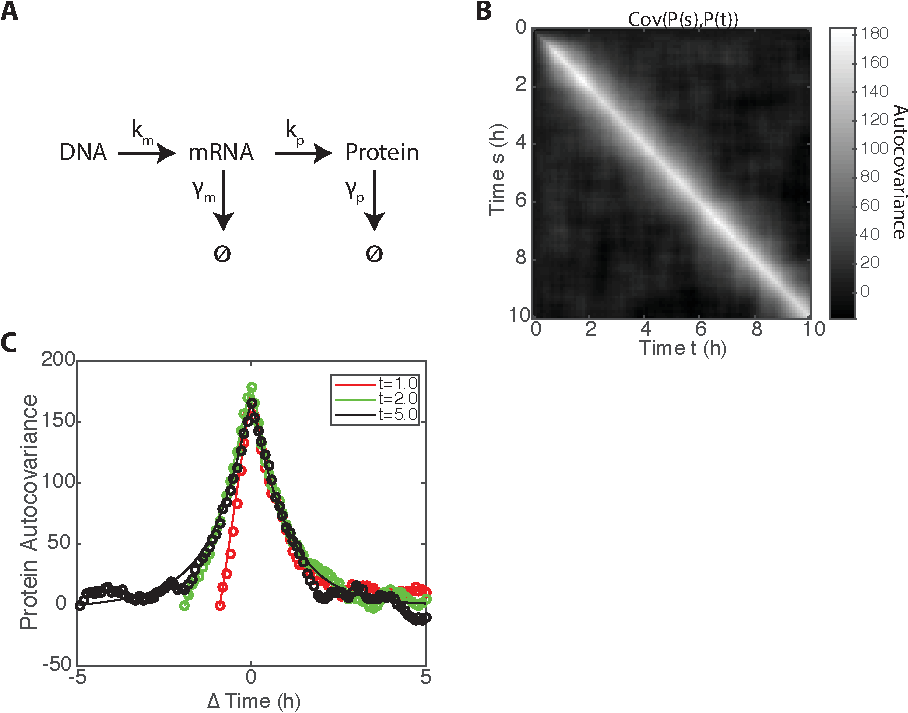
\includegraphics[width=0.8\textwidth]{Figures/S1.pdf}
\caption{\textbf{LNA accurately approximates a simple Birth-death model.} (A) mRNA and proteins are produced and degraded in a simple birth-death model.  (B) The protein autocovariance matrix, $\cov(P(s),P(t))$, estimated from empirical data. (C) Comparison of the LNA estimate and the empirical protein autocovariance at three time points. Estimates derived from SSA shown as circles, LNA as lines. }
\label{fig:birth-death-model}
\end{center}
\end{figure}

Stochastic simulations of the chemical reaction network were generated using the stochastic simulation algorithm \cite{Gillespie:1977uf} implemented in the StockKit~2.0 simulation framework \cite{Sanft:2011cj}.  For simulation, the parameters were set to $k_m=20$, $k_p=25$, $\gamma_m=10$ and $\gamma_p$=1.

\begin{table}
\centering
\caption{Reactions for a birth-death process}
\begin{tabular}{llcc}
$\mathcal{R}_1:$ & $\emptyset$ & $\overset{k_m} \longrightarrow$ & mRNA \nonumber\\
$\mathcal{R}_2:$ & mRNA & $\overset{\gamma_m} \longrightarrow $ & $\emptyset $\nonumber \\
$\mathcal{R}_3:$ & mRNA & $\overset{k_p} \longrightarrow $ & mRNA + Protein \nonumber \\
$\mathcal{R}_4:$ & Protein & $\overset{\gamma_p} \longrightarrow $ & $\emptyset$
\end{tabular}
\label{tab:BirthDeathReactions}
\end{table}


We performed exact simulation of the stochastic process and used LNA++ to compute the mean and temporal autocovariance of the proteins using the same model parameters.  For simplicity, and to replicate a typical fluorescence microscopy setup, only protein abundance is considered to be known.  The system size is set to $\Omega=1$ so that we can identify molecule numbers with molecular concentrations. For this simple system, the LNA agrees well with the exact stochastic simulations in terms of mean and variance (Figure~\ref{fig:birth-death-model}B) and the autocovariance (i.e.\ the cross-covariance of the protein only; Figures~\ref{fig:birth-death-model}C and~\ref{fig:birth-death-model}D). The autocovariance is shown at three sampled time points $(t=1.0, t=2.0, t=5.0)$, showing good qualitative agreement between the empirical covariance derived from 500 simulated SSA trajectories (Figure~\ref{fig:birth-death-model}E  circles), and from the LNA (Figure~\ref{fig:birth-death-model}E lines)\todo{Check missing subfigures D,E}.  In each case, the autocovariance is peaked at zero time lag, and decreases to zero in both directions, i.e. the correlation of fluctuations at a particular time point with future or past fluctuations decreases with increasing absolute time lag.

Next, we compute sensitivities of the mean protein copy number with respect to the model parameters using LNA++, and compare the computed results to a finite difference approximation.  We find that the sensitivity of the mean agrees exactly with a finite difference approximation for both first and second order sensitivities, see Figures~\ref{fig:mean-first-order-sensitivities} and~\ref{fig:mean-second-order-sensitivities}, respectively.  The first order sensitivity of the autocovariance also shows excellent agreement between the finite difference approximation and the analytical result from LNA++ (Figure~\ref{fig:autocovariance-first-order-sensitivities}).  Lastly, the second order sensitivities are difficult to compute robustly using finite differences, for example due to limited accuracy of the ODE solver. While this is generally the case, for this simple model the finite difference approximation still agrees reasonably well with the analytically computed sensitivities from LNA++ (Figure~\ref{fig:autocovariance-second-order-sensitivities}).


\begin{figure}[htbp]
\begin{center}
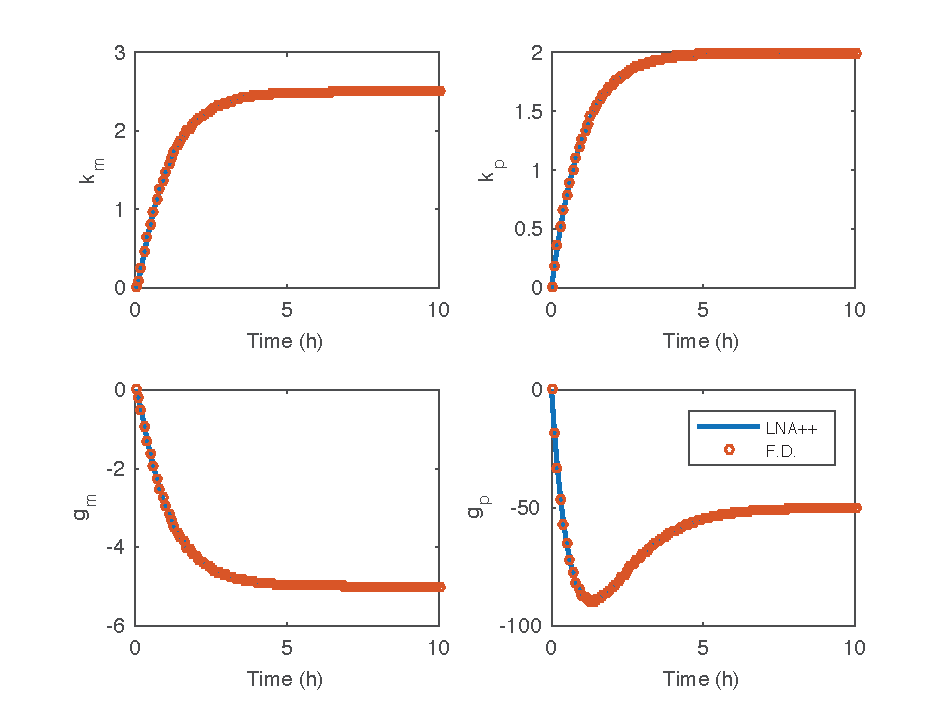
\includegraphics{Figures/S2.pdf}
\caption{\textbf{Comparison of the analytical first order sensitivity of mean protein concentration with respect to parameters ($\frac{\partial \phi}{\partial \theta_i}$) and the finite difference approximation.}}
\label{fig:mean-first-order-sensitivities}
\end{center}
\end{figure}

\begin{figure}[htbp]
\begin{center}
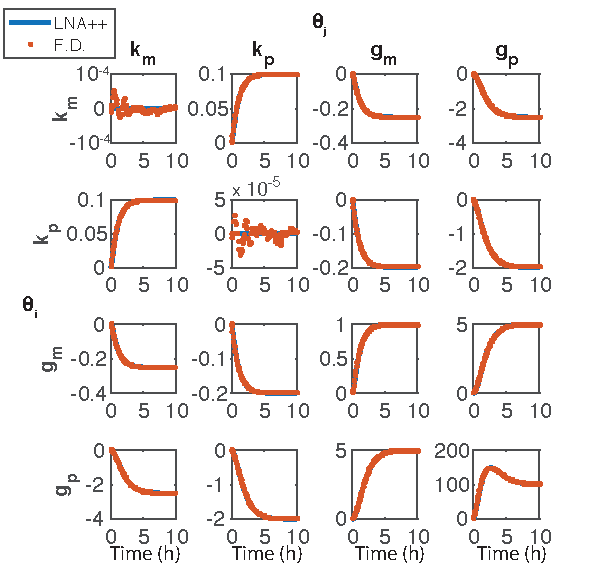
\includegraphics[width=\textwidth]{Figures/S3.pdf}
\caption{\textbf{Comparison of the analytical second order sensitivity of mean protein concentration with respect to parameters ($\frac{\partial^2 \phi}{\partial \theta_i \partial \theta_j} $) and the the finite difference approximation.}}
\label{fig:mean-second-order-sensitivities}
\end{center}
\end{figure}

\begin{figure}[htbp]
\begin{center}
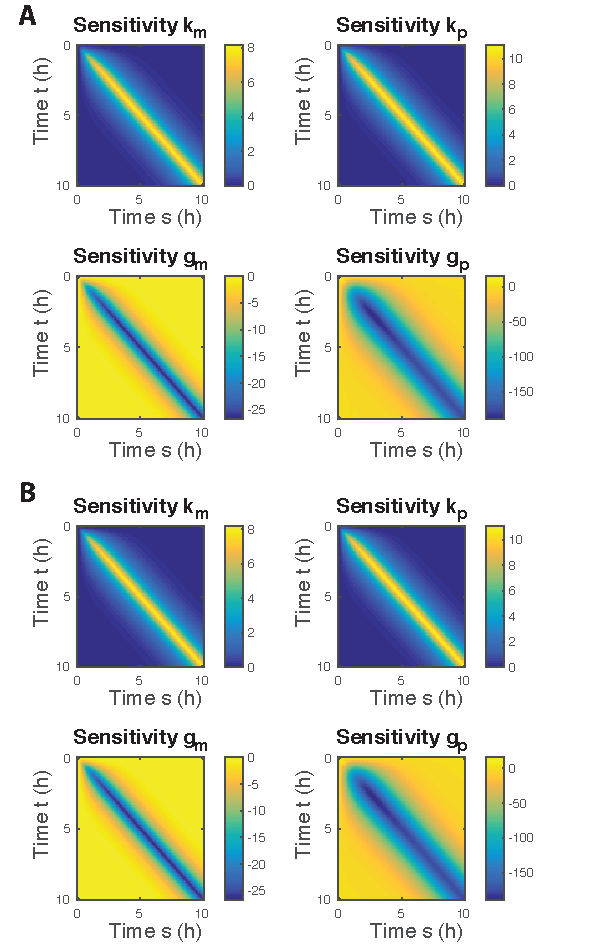
\includegraphics{Figures/S4.pdf}
\caption{\textbf{Comparison of the analytical  first order sensitivity of the protein autocovariance with respect to model parameters ($\frac{\partial \Sigma}{\partial \theta_i}$) and the finite difference approximation.} (A) Finite difference approximation. (B) Sensitivity analysis.}
\label{fig:autocovariance-first-order-sensitivities}
\end{center}
\end{figure}


\begin{figure}[htbp]
\begin{center}
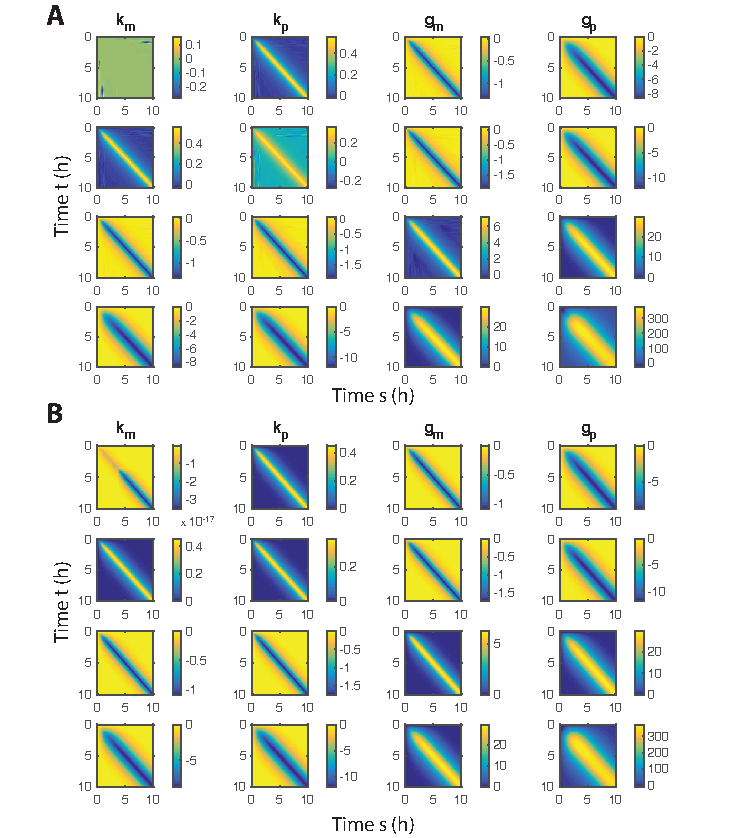
\includegraphics[width=0.85\textwidth]{Figures/S5.pdf}
\caption{\textbf{Comparison of the analytical second order sensitivities of the protein autocovariance with respect to model parameters ($\frac{\partial^2 \Sigma}{\partial \theta_i \partial \theta_j}$) and the finite difference approximation.} (A) Finite difference approximation. (B) Sensitivity analysis.}
\label{fig:autocovariance-second-order-sensitivities}
\end{center}
\end{figure}


We performed multi-start optimization in order to compare parameter inference with and without the analytical sensitivities. Performing 10 optimizations with randomly (Latin hypercube) chosen initial values for $(\gamma_m, \gamma_p)$ in the range $[1, 100] \times [0.01, 10]$ (the correct values of $k_m$ and $k_p$ are assumed to be known), we see that  the numerical optimization finds a continuum of local optima before terminating (Figure~\ref{fig:parameter-inference}A).  These optima have sometimes drastically different log-likelihood values (Figure~\ref{fig:parameter-inference}B) and differing values for the locally-optimal model parameters. By contrast, optimization performed using the analytical gradients computed using LNA++ shows excellent convergence to the same global optimum in each of the ten numerical optimizations (Figure~\ref{fig:parameter-inference}B).  The model parameters identified coincide with the true model parameters used to simulate the data (Figure~\ref{fig:parameter-inference}A), unlike the numerical optimization without sensitivities which shows substantial variation. We thus conclude that the first order sensitivities have provided a clear benefit for robust parameter optimization.

\begin{figure}[htbp!]
\begin{center}
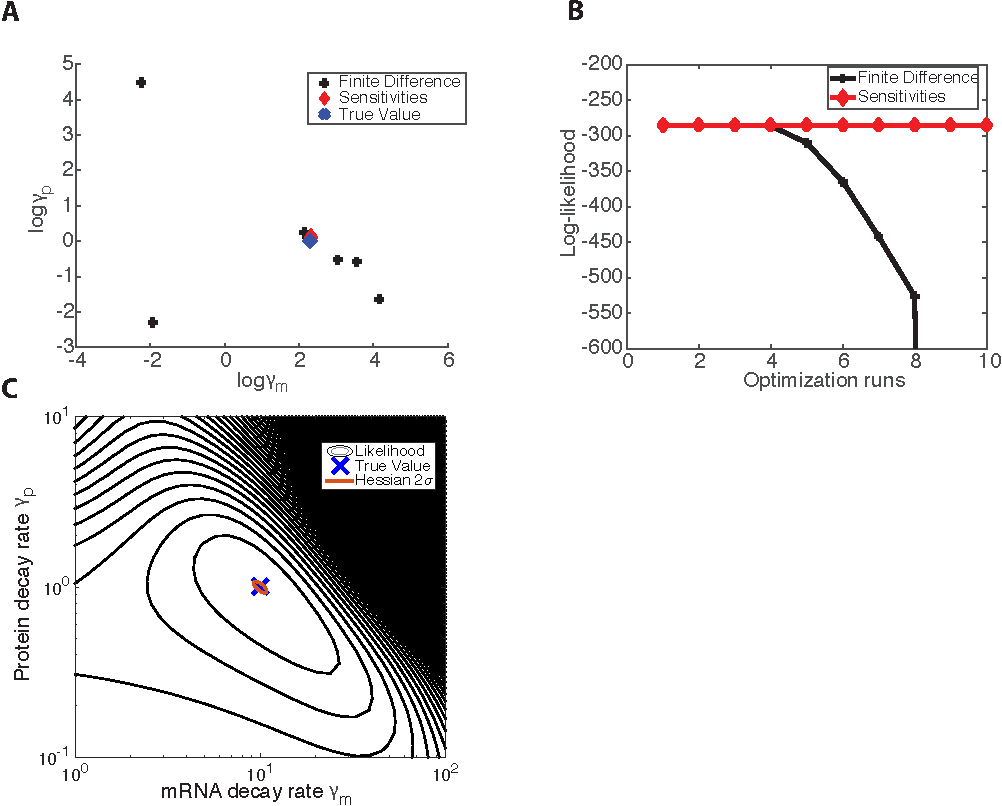
\includegraphics{Figures/S6.pdf}
\caption{\textbf{Analytic sensitivities greatly improve robustness of parameter inference.} (A) The MLE estimated using sensitivities. (B) The log-likelihood of the MLE for multiple optimization runs using sensitivities and a finite difference approximation. Optimization runs are sorted by their log-likelihoods. (C) The log-likelihood landscape of the degradation rates for mRNA and protein, estimated using the LNA, shows a clear optimum for the correct model parameters (contours indicated for $\log[-\ell(\bs \Theta)]$).  Using the second order sensitivities, it is possible to estimate the 95\% confidence interval for the model parameters (red).}
\label{fig:parameter-inference}
\end{center}
\end{figure}

Finally, we used LNA++ to evaluate the likelihood landscape for the simple birth-death model.  We fix the model parameters $k_m$ and $k_p$ to their correct values, and vary the parameters $\gamma_m$ and $\gamma_p$ over a large range encompassing the true parameters used for the stochastic simulations.  We find that the for this simple model, the mRNA and protein degradation rates are identifiable, showing a clear optimum at the true model parameters (Figure~\ref{fig:parameter-inference}C). Using the second order sensitivities to compute the 95\% confidence interval via the Laplace approximation~\eqref{eq:ConfidenceInterval}, we confirm that the parameters are indeed highly identifiable.

\subsection{Linear Chain}
To test the scaling performance of the LNA++ code, we implemented a series of models of increasing complexity.  Each model consists of a series of linear interconversions between species.  The simplest model consists of $n=3$ species $X_1$, $X_2$, and $X_3$, and the $2n$ reactions:
\begin{equation}
\begin{aligned}
\mathcal{R}_1: & \emptyset \overset{\alpha_1}{\longrightarrow} X_1  &
	\mathcal{R}_2: & X_1 \overset{\beta_1 }{\longrightarrow} \emptyset  \\
\mathcal{R}_3: & X_1 \overset{\alpha_{2}}{\longrightarrow} X_2 & 
	\mathcal{R}_4: & X_2 \overset{\beta_{2}}{\longrightarrow} X_1 \\
\mathcal{R}_5: & X_2 \overset{\alpha_{3}}{\longrightarrow} X_3 &
	R_6: & X_3 \overset{\beta_{3}}{\longrightarrow} X_2 
\end{aligned}
\end{equation}

In the same way we constructed models for $n=4\ldots 9$. In each case we assessed the ``offline cost'', i.e.\ the time necessary to compute the components of the LNA symbolically (a one time cost), and the ``online cost'', i.e.\ the time to evaluate the solution of the LNA (evaluated at each step of the optimization). We find that the offline cost grows with the model size, as many more equations needs to be solved (Figure~\ref{fig:computation-time-vs-model-size}A); offline costs include solving for components necessary for first and second order sensitivities.  We also estimate the online cost for the LNA solution both with and without sensitivities. The simulations were repeated 10 times each for different parameter sets with each individual parameter chosen randomly from the interval $[0,100]$, and initial conditions for each species chosen randomly from the interval $[0,1000]$, see Figure~\ref{fig:computation-time-vs-model-size}B. In each simulation, the same number of time points are used. Simulations were performed on a MacBook Pro laptop with a four core, 2.5GHz Intel i7 processor, and 16GB of RAM.  The run time grows quickly, especially when computing the second order sensitivities.  However, even with 9 species the run time without sensitivities is still a fraction of a second, and the run time including first order sensitivities approximately 1-2 seconds on average, thus suitable for parameter inference.

\begin{figure}[htb]
\begin{center}
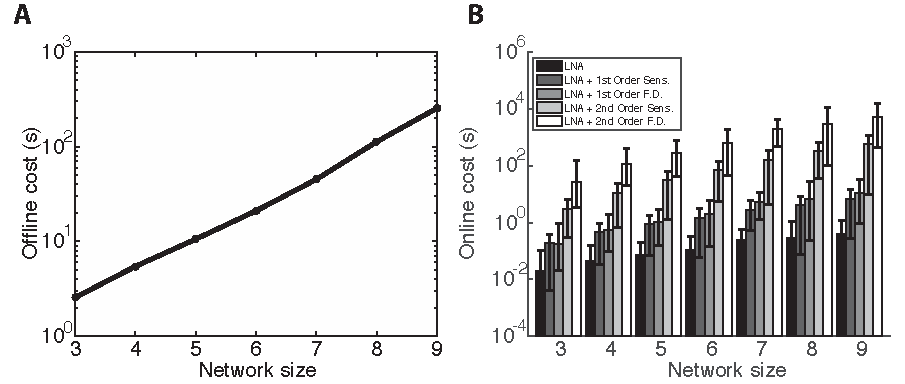
\includegraphics{Figures/S7.pdf}
\caption[labelInTOC]{\textbf{LNA++ offline and online computation cost versus model size.}  (A) The time to generate the Matlab executable (``offline cost''). (B) The median (1st and 3rd quantile) simulation run time (``online cost'') with randomly chosen model parameters ($n=10$). First and second order sensitivities computed using LNA++, and estimated for finite differences using a constant factor of $3n$ and $6n(3n-1)$ times the online cost of the LNA for network size $N$, for first order and second order finite differences, respectively.}
\label{fig:computation-time-vs-model-size}
\end{center}
\end{figure}

We compare the run time of the first and second order sensitivities to the estimated run time using finite differences.  Approximating the sensitivities using a forward difference scheme requires the evaluation of the function one additional time for each parameter (see Section \ref{sec:FirstOrderFD}). In the case of the linear chain model with $n$ species, there are $2n$ reactions rates and $n$ initial conditions (one for each species), leading to an additional $3n$ simulations necessary to approximate all first order sensitivities using finite differences. To approximate the second order sensitivities, an additional 4 evaluations of the function are necessary for each pair of model parameter/initial conditions (see Section \ref{sec:SecondOrderFD}), leading to a total of $4 \frac{N(N-1)}{2}$ additional evaluations of $f$ where $N$ is the number of parameters/initial conditions with respect to which to compute the second order sensitivities. As for the first order case $N=3n$, such that the second order finite difference requires a total of $2N(N-1) = 6n(3n-1)$ evaluations of $f$ in addition to those required by the first order finite difference approximation. Compared to the finite difference computation, the computation of the first order sensitivity computed using LNA++ was between 1.5 and 2.9 times faster, and the computation of the second order sensitivity between 11.4 and 20.5 times faster. Lastly, the sensitivities computed using the analytical expressions do not require \textit{a priori} knowledge of the length scale necessary for a robust finite difference approximation of the gradient, and are thus generally more robust and accurate. Run times for the finite difference approximation are estimated by multiplying the measured run times for the LNA without sensitivities by the factors $3n$ and $6n(3n-1)$ for the first and second order sensitivities, respectively.

In summary, LNA++ facilitates the automatic construction of LNAs and the corresponding forward sensitivity equations for small and medium-sized systems. The forward sensitivity equations provide a numerically more robust and computationally efficient means to calculate sensitivities than the finite difference approximation thus facilitating parameter inference and approximations of their corresponding confidence intervals.

%
%
\bibliographystyle{unsrt}
\bibliography{Documentation.bib}

\end{document}